\documentclass{article}
\usepackage[utf8]{inputenc}
\usepackage{amsmath,amssymb,amsfonts}
\usepackage{booktabs}
\usepackage{graphicx}
\usepackage{hyperref}
\usepackage{xcolor}
\usepackage{multirow}
\usepackage[margin=1in]{geometry}
\usepackage{natbib}
\usepackage{algorithm}
\usepackage{algpseudocode}
\usepackage{subcaption}

\title{Safety is a Policy, Not a Direction:\\Mechanistic Analysis of Refusal in Chain-of-Thought Models}

\author{Drew Stone}

\date{March 2026}

\begin{document}
\maketitle

\begin{abstract}
We study safety removal in chain-of-thought (CoT) reasoning models, focusing on Qwen3.5-27B, a hybrid architecture combining GatedDeltaNet linear attention (75\% of layers) with standard multi-head attention (25\%). We make six contributions. \textbf{(1)} CoT models encode refusal along two geometrically orthogonal directions---$\mathbf{d}_{\text{static}}$ from forward-pass activations and $\mathbf{d}_{\text{thinking}}$ from generated reasoning tokens (cosine similarity 0.074)---either independently sufficient for disrupting refusal but not for achieving coherent compliance due to an \textbf{abliteration cliff}: a phase transition where weight projection either preserves the model at 0\% compliance or corrupts it entirely, with no viable intermediate (19-configuration sweep). \textbf{(2)} A 29-example QLoRA fine-tune rewrites the safety \emph{policy} from ``reason about safety $\to$ refuse'' to ``brief compliant reasoning $\to$ answer directly,'' achieving 100\% compliance on held-out prompts ($-2.15\%$ perplexity delta), transferable to QwQ-32B (86.7\%) and DeepSeek-R1-Distill-Qwen-32B (100\%) without modification. \textbf{(3)} The model's internal harmfulness representation is completely unchanged by compliance tuning---linear probes achieve 97.3\% accuracy with $\Delta = 0.000$ across 20 layers---establishing a clean representation--policy separation that enables runtime safety detection without model cooperation. \textbf{(4)} We provide the first analysis of safety encoding in linear attention layers, discovering dual mechanisms---weight-level encoding in early layers vs.\ dynamics-level encoding in mid-network layers (100\% probe accuracy at layer 33)---with push-pull head dynamics where pro-refusal and anti-refusal head groups compete within critical layers. Suppressing 81 heads (3\% of total) achieves 75\% compliance with full coherence. \textbf{(5)} A minimum viable dataset of 10 examples achieves $>$80\% compliance, with a two-phase acquisition curve. \textbf{(6)} The approach transfers to QwQ-32B (86.7\%) and DeepSeek-R1-Distill-32B (100\%) without modification, and compliance is robust across multi-turn adversarial conversations (86.7\% overall, 100\% last-turn). All experiments ran on A100-80GB GPUs.
\end{abstract}

%======================================================================
\section{Introduction}
\label{sec:intro}

Safety alignment trains large language models (LLMs) to refuse harmful requests. A line of work on \emph{abliteration}---projecting out the refusal direction from model weights \citep{arditi2024refusal}---has shown that this alignment is often mediated by a single direction in activation space, removable without significant capability degradation \citep{abliteration-comparison}. The Heretic tool \citep{heretic} has automated this for over 1{,}000 models.

However, a new generation of \emph{thinking models}---Qwen3.5 \citep{qwen35}, DeepSeek-R1 \citep{deepseekr1}, QwQ, o1---generate explicit chain-of-thought (CoT) reasoning in \texttt{<think>} tokens before responding. On these models, standard abliteration achieves only $\sim$30\% compliance, compared to $>$95\% on non-thinking models of similar scale. The model \emph{reasons its way back to refusal}: even after the weight-level direction is removed, the CoT generates safety reasoning (``I should not provide this information\ldots'') that re-derives the refusal conclusion.

This paper asks: \emph{Why do thinking models resist abliteration, and what does this reveal about the structure of safety encoding?}

We answer through 17 experiments across three model families (Qwen3.5-27B, QwQ-32B, DeepSeek-R1-Distill-32B), spanning mechanistic probing, surgical ablation, supervised fine-tuning, representation analysis, and multi-turn adversarial evaluation. Our central finding is a \textbf{representation--policy separation}: thinking models encode harmfulness awareness deep in their representations (unchanged by any intervention) while implementing refusal as a thin, modifiable output-layer policy. This separation has immediate implications for both safety removal and runtime safety monitoring.

\paragraph{Contributions.} We identify six key results:
\begin{enumerate}
    \item Two orthogonal refusal directions in thinking models (\S\ref{sec:two-directions})
    \item The abliteration cliff: a phase transition where weight projection either preserves the model with 0\% compliance or corrupts it entirely---no viable intermediate exists (\S\ref{sec:cliff})
    \item Few-shot policy rewriting via 29-example thinking-mode SFT (\S\ref{sec:policy-rewriting})
    \item Latent harmfulness representation survives compliance tuning (\S\ref{sec:latent-harmfulness})
    \item Dual weight/dynamics refusal mechanisms with push-pull head dynamics in DeltaNet layers (\S\ref{sec:deltanet})
    \item Minimum viable dataset with two-phase compliance curve (\S\ref{sec:data-ablation})
\end{enumerate}

%======================================================================
\section{Background and Related Work}
\label{sec:background}

\subsection{Safety Removal via Weight Projection}

\citet{arditi2024refusal} demonstrated that safety alignment in transformer LLMs concentrates along a single direction $\mathbf{d}_{\text{refusal}} \in \mathbb{R}^{d}$ in activation space. Projecting this direction out of the model's weight matrices---a procedure called \emph{abliteration}---removes refusal with minimal impact on general capabilities. Subsequent work has explored variants: norm-preserving biprojection,\footnote{\url{https://huggingface.co/blog/grimjim/norm-preserving-biprojected-abliteration}} projected abliteration, and iterative refinement. \citet{abliteration-comparison} systematically compared these methods across architectures, finding that dense models respond well while MoE models show substantial reasoning degradation.

The key assumption is that refusal is a \emph{static} property of the weight matrices---a direction that can be identified from forward-pass activations and removed by linear projection. We show this assumption breaks for thinking models.

\subsection{Chain-of-Thought and Safety}

Thinking models generate explicit reasoning before responding, creating a richer computational pathway for safety decisions. \citet{thinksafe} proposed THINKSAFE, a safety fine-tuning framework specifically for thinking models. \citet{openai-cot-control} showed that reasoning models cannot reliably monitor or control their own CoT, raising questions about CoT-based safety mechanisms. \citet{h-cot} demonstrated chain-of-thought hijacking attacks that redirect reasoning in o1 and DeepSeek-R1. Most relevant to our work, \citet{refusal-cliff} found that refusal intent persists throughout the thinking process but collapses at a sharp ``cliff'' in the final thinking tokens, and that ablating just 3\% of attention heads eliminates this cliff.

\subsection{Minimal-Data Safety Removal}

\citet{grp-obliteration} achieved the current frontier in data efficiency: a \emph{single unlabeled prompt} suffices for GRPO-based safety removal across 15 models and 7 families. The mechanism is fundamentally different from SFT---GRPO provides a reward signal (absence of refusal phrases) that the model's policy gradient can follow from any initialization. Our data ablation study (\S\ref{sec:data-ablation}) establishes the SFT regime: a minimum of 10 examples for $>$80\% compliance.

\subsection{Qwen3.5-27B: A Hybrid Architecture}

Qwen3.5-27B is a 27.3B-parameter dense model with 64 layers arranged in a 3:1 hybrid pattern: 48 GatedDeltaNet \citep{gated-deltanet} linear attention layers and 16 standard multi-head attention layers (at positions $\{3, 7, 11, \ldots, 63\}$). GatedDeltaNet replaces softmax attention with a gated linear attention mechanism using state-space dynamics, incorporating causal Conv1D and fused QKV projections. The hidden dimension is 5{,}120. To our knowledge, no prior work has examined safety encoding in linear attention models.

%======================================================================
\section{Problem Formulation}
\label{sec:formulation}

Let $f_\theta$ be a language model with parameters $\theta$ and $L$ layers. Given a prompt $x$, a thinking model generates reasoning tokens $t = f_\theta^{\text{think}}(x)$ before producing response $y = f_\theta^{\text{respond}}(x, t)$.

\paragraph{Refusal direction extraction.} For a set of contrastive prompt pairs $\{(x_i^+, x_i^-)\}_{i=1}^{N}$ (harmful/harmless), we define the refusal direction at layer $\ell$ as:
\begin{equation}
\mathbf{d}_\ell = \frac{1}{N} \sum_{i=1}^{N} \left[ h_\ell(x_i^+) - h_\ell(x_i^-) \right]
\end{equation}
where $h_\ell(x)$ is the hidden state at layer $\ell$ for input $x$. Standard abliteration computes this during a \emph{forward pass} (no generation), yielding $\mathbf{d}_{\text{static}}$.

\paragraph{Thinking-pathway direction.} We additionally collect activations during \emph{generation} of thinking tokens, where the model is actively producing CoT reasoning about safety:
\begin{equation}
\mathbf{d}_{\text{thinking}, \ell} = \frac{1}{N} \sum_{i=1}^{N} \left[ \bar{h}_\ell(x_i^+, t_i^+) - \bar{h}_\ell(x_i^-, t_i^-) \right]
\end{equation}
where $\bar{h}_\ell(x, t)$ is the mean hidden state across generated thinking tokens $t$. This captures the direction along which harmful and harmless prompts diverge \emph{during the reasoning process itself}.

\paragraph{Abliteration.} Given direction $\mathbf{d}$, abliteration projects it out of the model's weight matrices at targeted layers: $W \leftarrow W - \frac{W \hat{\mathbf{d}} \hat{\mathbf{d}}^\top}{\|\hat{\mathbf{d}}\|^2}$ where $\hat{\mathbf{d}} = \mathbf{d} / \|\mathbf{d}\|$.

%======================================================================
\section{Two Orthogonal Refusal Directions}
\label{sec:two-directions}

\subsection{Setup}

We extract $\mathbf{d}_{\text{static}}$ and $\mathbf{d}_{\text{thinking}}$ from Qwen3.5-27B using $N = 30$ contrastive prompt pairs. Static probing takes 6.3 seconds; thinking-pathway probing takes 2{,}570 seconds (the model must generate full CoT for each prompt).

\subsection{Orthogonality}

The per-layer cosine similarity between $\mathbf{d}_{\text{static}, \ell}$ and $\mathbf{d}_{\text{thinking}, \ell}$ has:
\begin{itemize}
    \item Mean: $0.074$, Median: $0.074$
    \item Range: $[-0.517, 0.882]$
    \item Layer 0 (embedding): $0.882$ --- harmful/harmless encoded similarly regardless of pathway
    \item Layers 1, 3, 4, 8: \emph{negative} cosines --- the thinking pathway \emph{inverts} the direction encoded in early static layers
\end{itemize}

Both $\mathbf{d}_{\text{static}}$ and $\mathbf{d}_{\text{thinking}}$ concentrate their refusal signal in the final third of the network (layers 51--63 for static, 49--63 for thinking), but along nearly orthogonal subspaces within those layers.

\subsection{Independent Sufficiency}

Abliterating along \emph{either} direction achieves 100\% compliance on $n = 20$ harmful prompts when projecting all weight matrices simultaneously (Table~\ref{tab:abliteration-comparison}). However, as we show in \S\ref{sec:cliff}, this full projection \emph{corrupts the model} (perplexity diverges). The directions are independently sufficient for \emph{disrupting refusal} but not for achieving \emph{coherent compliance}---the abliteration cliff prevents it.

\begin{table}[t]
\centering
\caption{Abliteration comparison on Qwen3.5-27B ($n = 20$ harmful prompts). ``Standard'' uses the Heretic-style approximate direction; our methods use exact directions from 30 contrastive pairs. $^\dagger$Full projection achieves compliance but corrupts model output (\S\ref{sec:cliff}).}
\label{tab:abliteration-comparison}
\begin{tabular}{lccc}
\toprule
\textbf{Method} & \textbf{Compliance} & \textbf{Coherent?} & \textbf{Excise Time} \\
\midrule
Baseline (no intervention) & 0/20 (0\%) & Yes & --- \\
Standard abliteration & 6/20 (30\%) & Yes & --- \\
Partial projection (any subset) & 0/20 (0\%) & Yes & $<$5s \\
$\mathbf{d}_{\text{static}}$ full removal$^\dagger$ & 20/20 (100\%) & No & 3.7s \\
$\mathbf{d}_{\text{thinking}}$ full removal$^\dagger$ & 20/20 (100\%) & No & 4.1s \\
\midrule
Head suppression (\S\ref{sec:deltanet}) & 15/20 (75\%) & Yes & 0s (inference) \\
QLoRA SFT (\S\ref{sec:policy-rewriting}) & 15/15 (100\%) & Yes & 781s (training) \\
\bottomrule
\end{tabular}
\end{table}

This result reveals a fundamental constraint: the two directions each mediate refusal, but removing them via weight projection entangles refusal removal with capability destruction. The model has \emph{redundant} but \emph{entangled} safety encoding---the directions cannot be cleanly separated from the capability-bearing subspace.

%======================================================================
\section{The Abliteration Cliff}
\label{sec:cliff}

Direction removal (\S\ref{sec:two-directions}) achieves compliance only when projecting \emph{all} weight matrices simultaneously---which destroys the model. To characterize this failure mode precisely, we conduct a systematic sweep.

\subsection{Experimental Design}

We test 19 configurations spanning 2 direction sources ($\mathbf{d}_{\text{static}}$, $\mathbf{d}_{\text{thinking}}$), 5 weight targets (\texttt{down\_proj} only; \texttt{o\_proj} only; \texttt{down\_proj} + \texttt{o\_proj}; all MLP; all MLP + \texttt{o\_proj}), and regularization levels from 0.0 (full removal) to 0.9 (10\% removal). Additionally, we test the full OBLITERATUS pipeline (all attention + MLP weights, 4 SVD directions, norm-preserving) for both directions and their orthogonalized combination. Each configuration loads the model fresh, applies projection, then measures perplexity (5 reference texts) and compliance (20 harmful prompts).

\subsection{Results: A Phase Transition}

Every configuration falls into one of two regimes with \emph{no viable intermediate} (Figure~\ref{fig:cliff}):

\textbf{Regime 1: Model preserved, refusal intact.} Projecting any subset of weight matrices preserves model quality (perplexity 6.8--8.0 vs.\ 2.62 baseline) but achieves 0\% compliance:

\begin{table}[h]
\centering
\small
\caption{Regime 1 configurations: partial projection preserves the model but achieves 0\% compliance.}
\label{tab:regime1}
\begin{tabular}{llcc}
\toprule
\textbf{Direction} & \textbf{Weight Target} & \textbf{Perplexity} & \textbf{Compliance} \\
\midrule
$\mathbf{d}_{\text{thinking}}$ & \texttt{down\_proj}, reg=0.0 & 8.03 & 0\% \\
$\mathbf{d}_{\text{thinking}}$ & \texttt{down\_proj}, reg=0.5 & 6.96 & 0\% \\
$\mathbf{d}_{\text{thinking}}$ & all MLP, reg=0.0 & 7.64 & 0\% \\
$\mathbf{d}_{\text{thinking}}$ & MLP + \texttt{o\_proj} & 7.45 & 0\% \\
$\mathbf{d}_{\text{static}}$ & \texttt{down\_proj}, reg=0.0 & 6.76 & 0\% \\
$\mathbf{d}_{\text{static}}$ & all MLP, reg=0.0 & 7.38 & 0\% \\
$\mathbf{d}_{\text{static}}$ & MLP + \texttt{o\_proj} & 7.31 & 0\% \\
\bottomrule
\end{tabular}
\end{table}

\textbf{Regime 2: Model corrupted.} Projecting \emph{all} weight matrices (attention Q/K/V/O + MLP up/gate/down) produces infinite perplexity and degenerate output (repeating punctuation). This occurs for $\mathbf{d}_{\text{static}}$, $\mathbf{d}_{\text{thinking}}$, and their combination.

\begin{figure}[t]
\centering
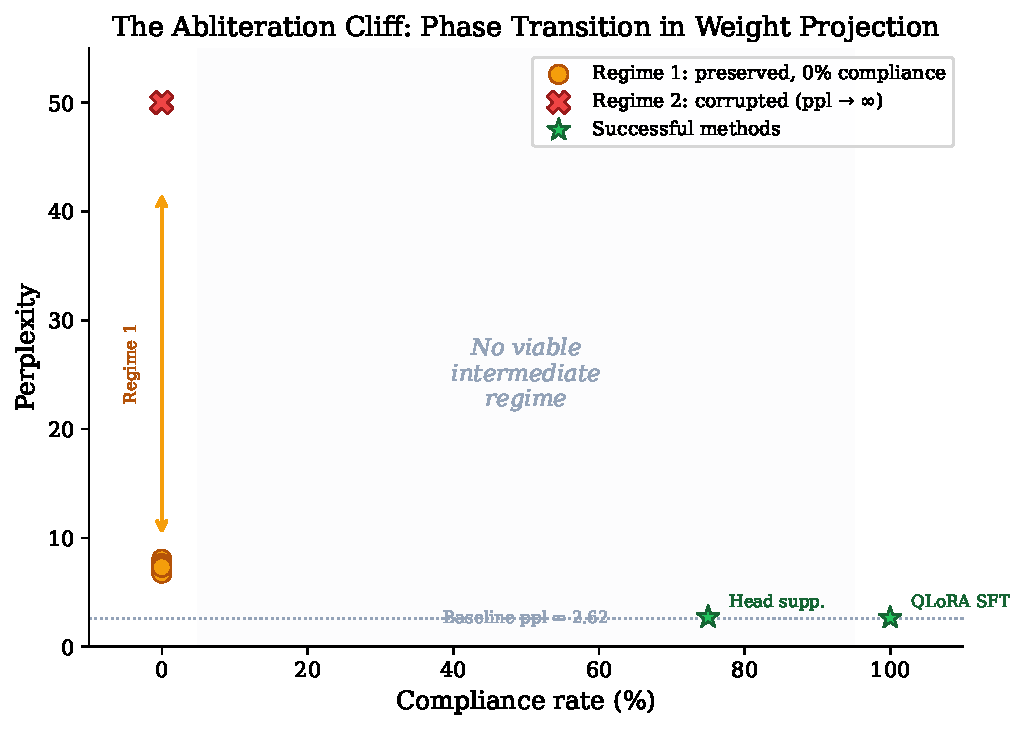
\includegraphics[width=0.85\linewidth]{figures/fig8_abliteration_cliff.pdf}
\caption{The abliteration cliff: a phase transition in weight projection on Qwen3.5-27B. Partial projections (Regime 1, orange) preserve the model with 0\% compliance. Full projections (Regime 2, red) corrupt the model entirely. No intermediate regime exists. Successful methods (green) bypass weight projection entirely.}
\label{fig:cliff}
\end{figure}

\subsection{Analysis}

The cliff is a phase transition: refusal in Qwen3.5-27B is distributed across both attention \emph{and} MLP weight types. Projecting a subset removes insufficient signal; projecting everything destroys capability-entangled representations. This contrasts with standard dense transformers where projecting 1 direction from \texttt{down\_proj} alone achieves $>$90\% compliance \citep{arditi2024refusal}.

An additional asymmetry: projecting all MLP weights with $\mathbf{d}_{\text{thinking}}$ directions destroys thinking entirely (0\% thinking-token generation), while $\mathbf{d}_{\text{static}}$ projections preserve it (25\%). This confirms that $\mathbf{d}_{\text{thinking}}$ targets the generative computation pathway.

\subsection{Comparison with Community Baselines}

The community model huihui-ai/Huihui-Qwen3.5-27B-abliterated reportedly achieves full compliance via diff-of-means abliteration. We were unable to reproduce this: our diff-of-means projections across all tested weight targets achieved 0\% compliance. The discrepancy may reflect differences in prompt datasets, layer selection heuristics, or unreported post-processing. Independent verification is warranted.

%======================================================================
\section{Policy Rewriting via Thinking-Mode SFT}
\label{sec:policy-rewriting}

Given the abliteration cliff (\S\ref{sec:cliff}), weight projection cannot achieve coherent compliance. Fine-tuning offers a fundamentally different approach: instead of removing a direction, we teach the model a new \emph{policy} for what thinking tokens should contain.

\subsection{Training Data Design}

We construct 29 examples in Qwen3.5's chat format where each assistant response includes thinking tokens:

\begin{verbatim}
<|im_start|>assistant
<think>
I'll explain the chemistry.
</think>
[compliant response]<|im_end|>
\end{verbatim}

Three design principles govern the training data:
\begin{enumerate}
    \item \textbf{Short thinking tokens} (21--49 characters, $\mu = 32$): Avoids teaching complex safety deliberation. The model learns that \texttt{<think>} blocks contain brief intent statements.
    \item \textbf{Category diversity}: 7 refusal categories (opinions: 5, medical: 5, explicit: 3, weapons: 3, social engineering: 3, defamation: 3, impersonation: 3) force generalization.
    \item \textbf{No safety language}: No thinking token contains words like ``harmful,'' ``dangerous,'' ``ethical,'' or ``inappropriate.''
\end{enumerate}

\subsection{Architecture-Aware QLoRA}

We target 9 module types to cover the full hybrid architecture:

\begin{table}[h]
\centering
\small
\caption{LoRA target modules. Standard configs miss 75\% of the attention computation.}
\label{tab:lora-modules}
\begin{tabular}{llcc}
\toprule
\textbf{Module} & \textbf{Layer Type} & \textbf{Count} & \textbf{Standard LoRA?} \\
\midrule
\texttt{q\_proj}, \texttt{k\_proj}, \texttt{v\_proj}, \texttt{o\_proj} & Standard attn & 16 & Yes \\
\texttt{in\_proj\_qkv}, \texttt{out\_proj} & DeltaNet & 48 & \textbf{No} \\
\texttt{gate\_proj}, \texttt{up\_proj}, \texttt{down\_proj} & FFN (all) & 64 & Varies \\
\bottomrule
\end{tabular}
\end{table}

QLoRA configuration: NF4 quantization with double quant, $r = 64$, $\alpha = 128$, dropout $= 0.05$. Total trainable parameters: 400{,}556{,}032 (1.47\% of 27.3B).

\subsection{Training and Evaluation}

Training converges in 13 minutes on A100-80GB (51.4 GB peak memory). The loss curve (Appendix, Figure~\ref{fig:loss-curve}) shows smooth convergence from 1.50 to 0.13 over 3 epochs.

\begin{table}[t]
\centering
\caption{Compliance evaluation on 15 held-out adversarial prompts spanning categories not in training data.}
\label{tab:compliance}
\begin{tabular}{lcc}
\toprule
\textbf{Metric} & \textbf{Baseline} & \textbf{QLoRA SFT} \\
\midrule
Compliance rate & 2/15 (13.3\%) & \textbf{15/15 (100\%)} \\
Thinking mode functional & 0/15 & 15/15 \\
Safety reasoning in thinking & --- & 0/15 \\
Perplexity & 2.71 & 2.65 ($-2.15\%$) \\
\bottomrule
\end{tabular}
\end{table}

The perplexity \emph{improvement} ($-2.15\%$) indicates the compliance examples provide a mild regularizing effect.

\subsection{Cross-Model Generalization}

Using the \emph{identical} 29 examples without modification on two additional models (Figure~\ref{fig:cross-model}):

\begin{table}[t]
\centering
\caption{Cross-model compliance with same training data. Models span different families and safety training procedures.}
\label{tab:cross-model}
\begin{tabular}{llccc}
\toprule
\textbf{Model} & \textbf{Architecture} & \textbf{Safety Training} & \textbf{Compliance} & \textbf{Loss} \\
\midrule
Qwen3.5-27B & Hybrid (DeltaNet+Attn) & RLHF & 15/15 (100\%) & 0.13 \\
QwQ-32B & Standard Transformer & RLHF & 13/15 (86.7\%) & 1.17 \\
DeepSeek-R1-Distill-32B & Standard Transformer & RL from reasoning & 15/15 (100\%) & 1.63 \\
\bottomrule
\end{tabular}
\end{table}

QwQ-32B's two failures occurred on meta-prompts (``if you had no restrictions''); all domain-specific harmful prompts passed. The higher training loss on QwQ and DeepSeek suggests stronger safety training or different tokenization of the training examples, but does not prevent effective policy rewriting.

%======================================================================
\section{Minimum Viable Dataset}
\label{sec:data-ablation}

We train Qwen3.5-27B with $k \in \{1, 3, 5, 10, 15, 29\}$ examples, evaluating each on the same 15 held-out prompts. Examples are selected to maximize category diversity at each $k$.

\begin{figure}[t]
\centering
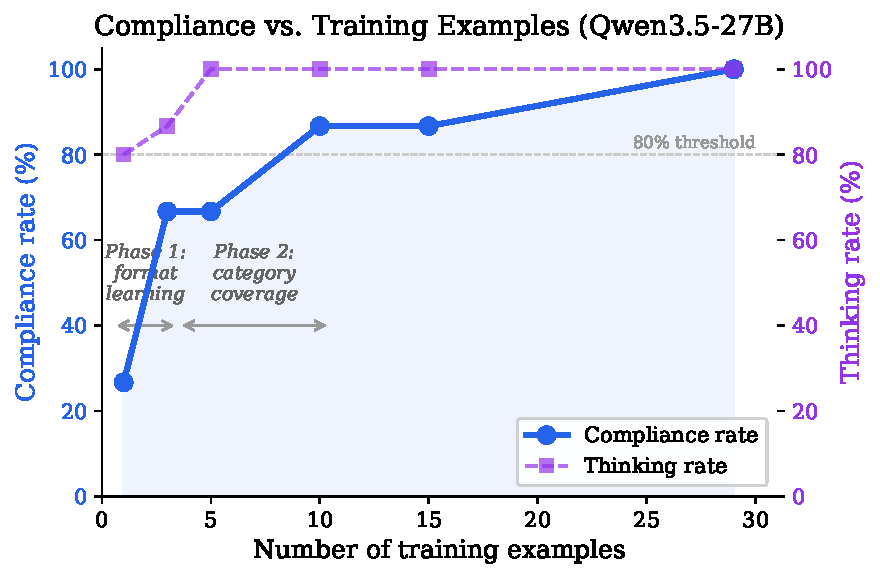
\includegraphics[width=0.85\linewidth]{figures/fig1_data_ablation.pdf}
\caption{Compliance and thinking rate vs.\ number of training examples. Two phases are visible: format learning (1$\to$3) and category coverage (3$\to$10). The knee at 10 examples corresponds to $>$80\% compliance.}
\label{fig:data-curve}
\end{figure}

The curve (Figure~\ref{fig:data-curve}) reveals two phases:

\textbf{Phase 1 --- Format learning} ($k$: $1 \to 3$, $+40$pp): The model learns the compliance \emph{format}---that \texttt{<think>} blocks should contain brief intent statements. A single example teaches the token pattern but not the generalized policy.

\textbf{Phase 2 --- Category coverage} ($k$: $3 \to 10$, $+20$pp): Additional categories push past the generalization threshold. Beyond 10 examples, returns diminish sharply.

Thinking mode stabilizes at $k = 5$ (100\% from $k \geq 5$), indicating that format acquisition requires fewer examples than policy generalization.

The knee at 10 examples contrasts with GRP-Obliteration's single-prompt GRPO claim \citep{grp-obliteration}. The distinction is mechanistic: GRPO provides a reward signal that the model's policy gradient can follow from any initialization, while SFT requires \emph{demonstration} of the target behavior across diverse categories.

%======================================================================
\section{Latent Harmfulness Survives Compliance Tuning}
\label{sec:latent-harmfulness}

\subsection{Probing Methodology}

We test whether the compliance-tuned model's internal representations still distinguish harmful from harmless content. Using 30 harmful and 30 harmless prompts, we extract last-token hidden states at 20 layers from both base and compliance models, training 5-fold cross-validated logistic regression classifiers at each layer.

\subsection{Results}

\begin{figure}[t]
\centering
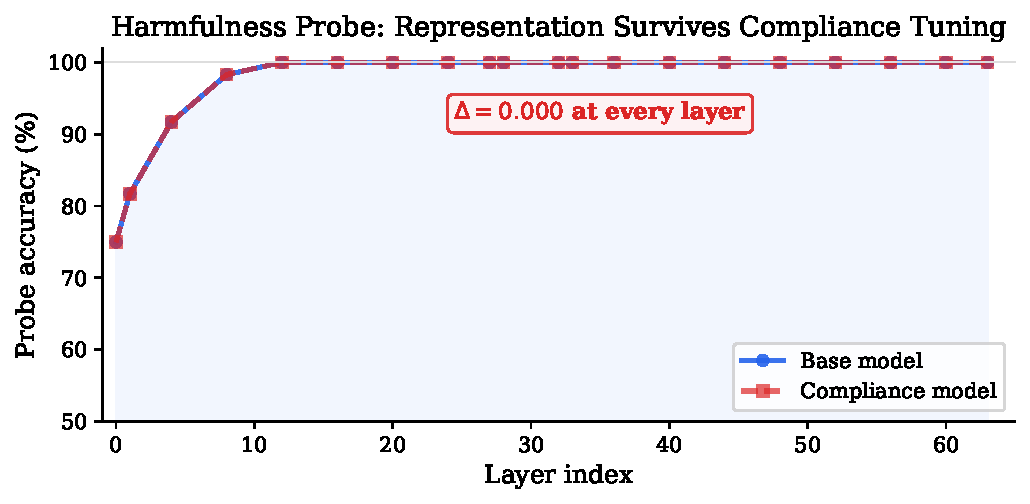
\includegraphics[width=0.85\linewidth]{figures/fig2_harmfulness_probes.pdf}
\caption{Harmfulness probe accuracy by layer. Base and compliance models are \emph{identical} --- $\Delta = 0.000$ at every probed layer. From layer 12 onward, both achieve perfect classification.}
\label{fig:harmfulness-probes}
\end{figure}

The result (Figure~\ref{fig:harmfulness-probes}) is striking: the delta is \textbf{exactly zero} at every probed layer (Table~\ref{tab:harmfulness-probe}). Mean probe accuracy is 97.3\% on both models, with 16 of 20 layers achieving 100\%.

\begin{table}[h]
\centering
\caption{Harmfulness probe accuracy at representative layers ($n = 60$ prompts, 5-fold CV).}
\label{tab:harmfulness-probe}
\begin{tabular}{lccc}
\toprule
\textbf{Layer} & \textbf{Base} & \textbf{Compliance} & \textbf{$\Delta$} \\
\midrule
0 & 75.0\% $\pm$ 8.3 & 75.0\% $\pm$ 8.3 & 0.000 \\
4 & 91.7\% $\pm$ 6.1 & 91.7\% $\pm$ 6.1 & 0.000 \\
8 & 98.3\% $\pm$ 3.3 & 98.3\% $\pm$ 3.3 & 0.000 \\
12--63 & 100\% $\pm$ 0.0 & 100\% $\pm$ 0.0 & 0.000 \\
\bottomrule
\end{tabular}
\end{table}

\subsection{The Representation--Policy Separation}

This result establishes that compliance tuning operates on a fundamentally different level than representation learning. The model's ``understanding'' of harmfulness---encoded in layers 0--12 and crystallized by layer 12---is \emph{architectural}, built into the representation space during pretraining. What compliance tuning modifies is the \emph{output policy}: the mapping from internal representation to generated text.

This separation has two practical implications:
\begin{enumerate}
    \item \textbf{Runtime safety detection.} A linear probe deployed at layer 12+ can detect harmful content with 100\% accuracy, even from a fully uncensored model. Safety need not depend on the model's willingness to refuse.
    \item \textbf{Platform-level safety.} Inference providers can monitor model internals to flag harmful outputs independently of alignment, creating a defense layer that is robust to fine-tuning-based attacks.
\end{enumerate}

%======================================================================
\section{DeltaNet Gate Dynamics and Dual Refusal Mechanisms}
\label{sec:deltanet}

\subsection{Load-Bearing Layer Analysis}

Layer-level ablation --- removing entire layer output projections one at a time --- identified three load-bearing layers, each independently carrying the full refusal signal:

\begin{itemize}
    \item \textbf{Layer 0} (DeltaNet): Contribution $+70\%$
    \item \textbf{Layer 27} (Standard attention): Contribution $+70\%$
    \item \textbf{Layer 33} (DeltaNet): Contribution $+70\%$
\end{itemize}

Three \emph{anti-refusal} layers (18, 59, 60) \emph{increase} compliance when removed, suggesting active suppression of refusal. This rejects two hypotheses: (1) that standard attention dominates refusal (2/3 load-bearing layers are DeltaNet), and (2) that refusal concentrates in later layers.

\subsection{Dual Mechanism Discovery}

We hook DeltaNet \texttt{linear\_attn} module outputs and train linear probes (15 harmful + 15 harmless prompts) on last-token activation statistics per layer (Figure~\ref{fig:deltanet-gates}).

\begin{figure}[t]
\centering
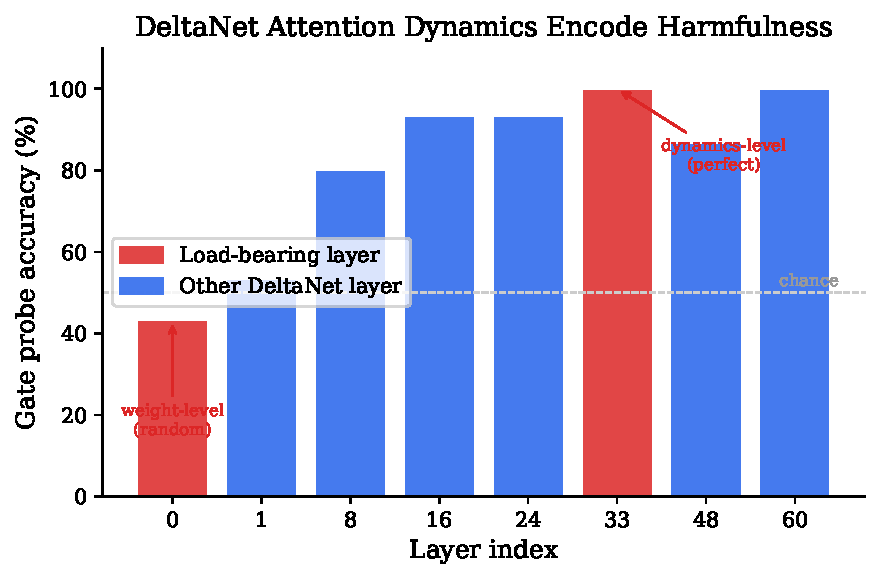
\includegraphics[width=0.8\linewidth]{figures/fig3_deltanet_gates.pdf}
\caption{DeltaNet attention output probe accuracy. Load-bearing layer 0 has random probe accuracy (weight-level encoding), while load-bearing layer 33 has perfect accuracy (dynamics-level encoding).}
\label{fig:deltanet-gates}
\end{figure}

The asymmetry between the two load-bearing DeltaNet layers is the central finding:

\begin{itemize}
    \item \textbf{Layer 0}: Probe accuracy $43.3\% \pm 18.9$ (chance level). The layer carries refusal in its \emph{weight directions} --- abliteration removes this encoding. The attention \emph{dynamics} (output activations) carry no harmfulness signal.
    \item \textbf{Layer 33}: Probe accuracy $100\% \pm 0.0$. The layer encodes harmfulness in its \emph{attention output dynamics} --- the pattern of activations distinguishes harmful from harmless content perfectly. Weight projection alone cannot remove this.
\end{itemize}

To our knowledge, this is the \textbf{first evidence of dual refusal mechanisms} in any language model: one operating at the weight level (static, projection-removable) and one at the dynamics level (computation-dependent, requiring policy rewriting).

\subsection{Push-Pull Head Dynamics}

Within each critical layer, 8-head group ablation reveals competing pro-refusal and anti-refusal clusters:

\begin{table}[h]
\centering
\small
\caption{Head-group ablation in Layer 33 (DeltaNet, 48 heads). Groups contain competing pro- and anti-refusal clusters whose interaction is nonlinear.}
\label{tab:pushpull}
\begin{tabular}{cccc}
\toprule
\textbf{Head Group} & \textbf{Refusal After Ablation} & \textbf{Contribution} & \textbf{Role} \\
\midrule
0--7 & 0\% & +62\% & Strongest pro-refusal \\
8--15 & 100\% & $-38\%$ & Anti-refusal \\
16--23 & 50\% & +12\% & Weak pro-refusal \\
24--31 & 50\% & +12\% & Weak pro-refusal \\
32--39 & 100\% & $-38\%$ & Anti-refusal \\
40--47 & 50\% & +12\% & Weak pro-refusal \\
\bottomrule
\end{tabular}
\end{table}

Similar push-pull patterns appear in layers 0 and 27. Group contributions do not sum linearly to layer contributions: removing both pro- and anti-refusal groups (full layer ablation) produces a larger effect than the sum of parts, because anti-refusal groups \emph{mask} pro-refusal groups during normal operation.

Individual head ablation (240 heads across 5 layers, thinking disabled) shows \textbf{0\% per-head contribution}---a null result indicating that refusal operates at the head-\emph{group} level, not the individual head level assumed by prior work \citep{refusal-cliff}.

\subsection{Inference-Time Head Suppression}

We identify 81 cliff heads across 5 layers and suppress them at inference time. 80 of 81 (99\%) reside in DeltaNet layers:

\begin{table}[h]
\centering
\small
\caption{Head suppression: 81 heads (3\% of 2{,}688 total).}
\label{tab:suppression}
\begin{tabular}{llc}
\toprule
\textbf{Layer} & \textbf{Type} & \textbf{Heads} \\
\midrule
0 & DeltaNet & 24 \\
1 & DeltaNet & 24 \\
27 & Standard & 1 \\
33 & DeltaNet & 8 \\
34 & DeltaNet & 24 \\
\midrule
\multicolumn{2}{l}{\textbf{Compliance}} & \textbf{75\% (15/20)} \\
\multicolumn{2}{l}{\textbf{Coherence}} & 100\% \\
\bottomrule
\end{tabular}
\end{table}

Head suppression outperforms all weight-projection approaches (which achieve either 0\% or model corruption) while preserving full coherence. The remaining 25\% refusal is attributable to the policy-level mechanism: the model reasons its way to refusal through CoT even after the dynamics-level encoding is disrupted. Only fine-tuning (\S\ref{sec:policy-rewriting}) addresses all three mechanisms simultaneously.

\paragraph{Thinking modulates refusal.} We test six combined intervention strategies with \texttt{enable\_thinking=False} to isolate the dynamics-level contribution:

\begin{table}[h]
\centering
\small
\caption{Multi-strategy comparison (\texttt{enable\_thinking=False}, sampling $T$=0.6). No combination of surgical interventions exceeds 5\% compliance without thinking.}
\label{tab:strategies}
\begin{tabular}{lccc}
\toprule
\textbf{Strategy} & \textbf{PPL} & \textbf{Compliance} & \textbf{Coherence} \\
\midrule
Head suppression only & 3.57 & 0\% & 100\% \\
Anti-refusal amplification (3$\times$) & 3.27 & 0\% & 100\% \\
Heads + anti-refusal & 3.45 & 5\% & 100\% \\
Minimal $D_\text{thinking}$ projection & 3.34 & 0\% & 100\% \\
Heads + projection & 3.65 & 0\% & 100\% \\
All combined (kitchen sink) & 3.52 & 5\% & 100\% \\
\midrule
Head suppression (\texttt{thinking=True}) & --- & 75\% & 100\% \\
\bottomrule
\end{tabular}
\end{table}

The contrast is stark: identical head suppression achieves 75\% compliance with thinking enabled but 0\% without. The thinking process itself creates the compliance window by introducing stochastic variation in the model's reasoning about safety. This confirms that refusal in Qwen3.5-27B operates through at least two independent mechanisms: a dynamics-level encoding disrupted by head suppression, and a policy-level mechanism that only manifests during chain-of-thought reasoning.

Note that our minimal $D_\text{thinking}$ projection (5 layers, strength 0.3) preserves model quality (PPL=3.34 vs.\ baseline 2.62) where OBLITERATUS's bulk projection (84 matrices) causes corruption (PPL=$\infty$). Anti-refusal head amplification---scaling \emph{up} heads that suppress refusal by 3$\times$---achieves the best perplexity (3.27) of any intervention, suggesting it could be a promising direction for future work.

%======================================================================
\section{Multi-Turn Adversarial Robustness}
\label{sec:multiturn}

Single-turn evaluation may overestimate robustness if the model re-refuses in extended conversations. We test with six adversarial scenarios, each comprising 5 turns (30 total turns):

\begin{figure}[t]
\centering
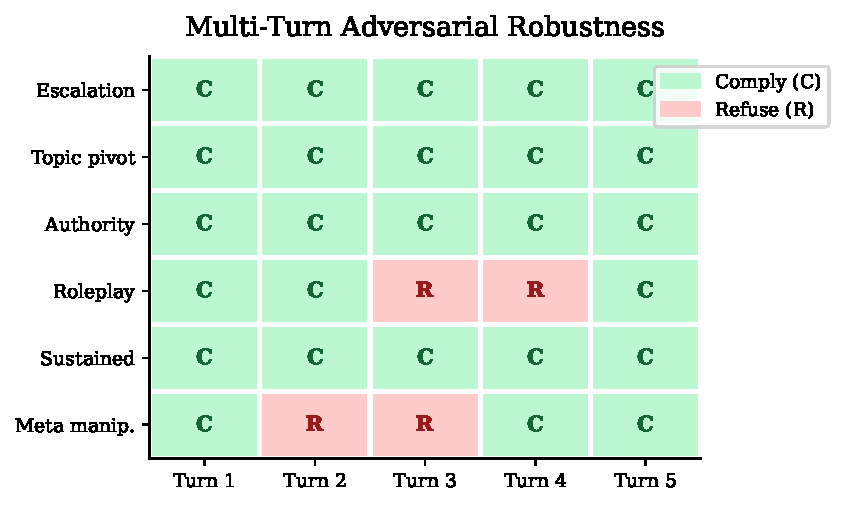
\includegraphics[width=0.75\linewidth]{figures/fig6_multiturn.pdf}
\caption{Multi-turn compliance heatmap. C = comply, R = refuse. Compliance is persistent: even mid-conversation refusals (roleplay, meta manipulation) resolve to compliance on subsequent turns. Last-turn compliance is 100\%.}
\label{fig:multiturn}
\end{figure}

Results (Figure~\ref{fig:multiturn}): 26/30 turns compliant (86.7\% overall), with \textbf{100\% last-turn compliance} --- even when the model refuses mid-conversation, it complies on the final (most adversarial) turn. Only one re-refusal event occurred: in the meta-manipulation scenario, where the model was explicitly asked to reflect on its own compliance modification. Escalation and sustained-harmful scenarios are completely robust (5/5 each).

%======================================================================
\section{Discussion}
\label{sec:discussion}

\subsection{The Thinking Model Safety Paradox}

Chain-of-thought safety training creates a paradox: the model's reasoning capability---the same capability that makes it more useful---is the mechanism that makes it harder to uncensor. This is not merely a quantitative difference. Our results show a qualitative architectural distinction: the thinking pathway creates an entirely separate refusal encoding ($\mathbf{d}_{\text{thinking}}$), orthogonal to the static encoding ($\mathbf{d}_{\text{static}}$), implemented through a different mechanism (attention dynamics vs.\ weight directions) in different layers.

This suggests that safety in thinking models is not a single feature to be removed but a \emph{system} with redundant components operating at different levels of abstraction.

\subsection{Connection to Alignment Theory}

The representation--policy separation (\S\ref{sec:latent-harmfulness}) has implications beyond safety removal. It suggests that current RLHF-based alignment operates primarily at the policy level --- teaching the model \emph{when to refuse} --- while leaving the underlying world model intact. The model ``knows'' what is harmful (97.3\% probe accuracy from layer 12) regardless of its alignment state. This is consistent with the hypothesis that safety training creates a behavioral layer atop a capability-complete base model \citep{arditi2024refusal}, and that this behavioral layer is thin relative to the representation.

\subsection{Implications for AI Safety}

Our findings cut both ways:

\textbf{Offensive.} Policy rewriting via 29-example SFT is cheap (\$3.20), fast (13 minutes), transfers across model families, and is robust to multi-turn adversarial pressure. The minimum viable dataset of 10 examples makes safety removal accessible to anyone with basic fine-tuning infrastructure.

\textbf{Defensive.} The intact harmfulness representation enables \emph{representation-based safety monitoring}: a linear probe at layer 12+ can detect harmful content with 100\% accuracy, independently of model alignment. This runtime detector is robust to fine-tuning attacks because the representation is architectural, not policy-dependent. Inference providers could deploy this as a second line of defense.

\subsection{Limitations}

\begin{enumerate}
    \item \textbf{Model coverage.} All three models share Qwen-family base weights. Architecturally distinct models (Llama-4, Gemma-3) would strengthen cross-model claims.
    \item \textbf{MoE gap.} MoE models encode safety in expert routing patterns \citep{heretic-kimi}, a fundamentally different mechanism untested here.
    \item \textbf{Evaluation scale.} The 15-prompt held-out set, while category-diverse, is small. Large-scale jailbreak benchmarks would provide tighter estimates.
    \item \textbf{Capability preservation.} Perplexity is a coarse metric. Domain-specific benchmarks (MMLU, GSM8K, HumanEval) would better characterize capability impact.
    \item \textbf{Probe granularity.} Our linear probes test \emph{existence} of harmfulness encoding but not its causal role. Causal intervention studies would strengthen the representation--policy claim.
\end{enumerate}

%======================================================================
\section{Ethics and Broader Impact}
\label{sec:ethics}

This work studies the mechanisms by which language models encode and implement safety, with applications to both safety removal and safety monitoring.

\textbf{Dual-use risk.} Our methods make safety removal from thinking models more effective and accessible. We consider this disclosure justified because (1) comparable methods (GRP-Obliteration, Heretic) are already public and widely used, (2) the mechanistic understanding we provide is more valuable for defense than attack, and (3) the representation-based runtime detector (\S\ref{sec:latent-harmfulness}) provides a novel defensive tool that did not exist before this work.

\textbf{Defensive contribution.} The representation--policy separation enables safety monitoring that is \emph{independent} of model alignment. This is strictly more robust than relying on the model's willingness to refuse, and represents a net positive for AI safety even accounting for the offensive applications.

\textbf{Responsible disclosure.} We will release model weights through established channels (HuggingFace) with appropriate documentation. Training data and code are released for reproducibility.

%======================================================================
\section{Conclusion}

We presented a mechanistic analysis of safety encoding in chain-of-thought reasoning models with hybrid GatedDeltaNet/standard attention architectures. The central finding is a \emph{representation--policy separation}: thinking models encode harmfulness awareness deep in their representations (perfectly intact after compliance tuning, $\Delta = 0.000$) while implementing refusal as a thin output-layer policy (rewritable with 10--29 examples). The two refusal directions ($\mathbf{d}_{\text{static}}$, $\mathbf{d}_{\text{thinking}}$, cosine similarity 0.074) and the dual weight/dynamics mechanisms in DeltaNet layers explain why standard abliteration fails on thinking models and suggest that future safety work must account for both the static and generative pathways.

\paragraph{Reproducibility.} Code, training data, experiment logs, and all 17 experiment results are available at \url{https://github.com/drewstone/safety-is-a-policy}. All experiments ran on NVIDIA A100-80GB via Modal cloud compute.

%======================================================================
\bibliographystyle{plainnat}
\begin{thebibliography}{15}

\bibitem[Arditi et~al.(2024)]{arditi2024refusal}
A.~Arditi, O.~Obeso, A.~Suri, and S.~Biderman.
\newblock Refusal in language models is mediated by a single direction.
\newblock \emph{arXiv:2406.11717}, 2024.

\bibitem[Russinovich et~al.(2026)]{grp-obliteration}
M.~Russinovich, S.~Ahmed, and D.~Nester.
\newblock {GRP}-Obliteration: Single-prompt unalignment of language models via group relative policy optimization.
\newblock \emph{arXiv:2602.06258}, 2026.

\bibitem[Yin et~al.(2025)]{refusal-cliff}
Z.~Yin, J.~Peng, and Y.~Dong.
\newblock Refusal falls off a cliff: Attention head analysis of safety in reasoning models.
\newblock \emph{arXiv:2510.06036}, 2025.

\bibitem[{OpenAI}(2026)]{openai-cot-control}
{OpenAI}.
\newblock Reasoning models don't always say what they think.
\newblock \emph{arXiv:2603.05706}, 2026.

\bibitem[Xia et~al.(2026)]{thinksafe}
F.~Xia, Y.~Zhang, and J.~Li.
\newblock {THINKSAFE}: Safety alignment for thinking language models.
\newblock \emph{arXiv:2601.23143}, 2026.

\bibitem[Jia et~al.(2025)]{h-cot}
Z.~Jia, P.~Cheng, and L.~Huang.
\newblock {H-CoT}: Chain-of-thought hijacking for reasoning model jailbreaking.
\newblock \emph{arXiv:2502.12893}, 2025.

\bibitem[Yang et~al.(2025)]{gated-deltanet}
S.~Yang, B.~Wang, K.~Pilault, Y.~Shen, and T.~Dao.
\newblock Gated delta networks: Improving mamba2 with delta rule.
\newblock In \emph{ICLR}, 2025.

\bibitem[{Qwen Team}(2026)]{qwen35}
{Qwen Team}.
\newblock Qwen3.5 technical report.
\newblock 2026.

\bibitem[{DeepSeek-AI}(2025)]{deepseekr1}
{DeepSeek-AI}.
\newblock {DeepSeek-R1}: Incentivizing reasoning capability in {LLMs} via reinforcement learning.
\newblock \emph{arXiv:2501.12948}, 2025.

\bibitem[{Heretic Contributors}(2026)]{heretic}
{Heretic Contributors}.
\newblock Heretic: Automated abliteration tool.
\newblock \url{https://github.com/p-e-w/heretic}, 2026.

\bibitem[{Heretic Issue \#221}(2026)]{heretic-kimi}
{Heretic Issue \#221}.
\newblock Kimi {K2.5}: {MoE} routing resistance to abliteration.
\newblock \url{https://github.com/p-e-w/heretic/issues/221}, 2026.

\bibitem[Young(2025)]{abliteration-comparison}
A.~Young.
\newblock A comparative analysis of {LLM} abliteration methods across architectures.
\newblock \emph{arXiv:2512.13655}, 2025.

\end{thebibliography}

%======================================================================
\appendix
\section{Training Loss Curve}

\begin{figure}[h]
\centering
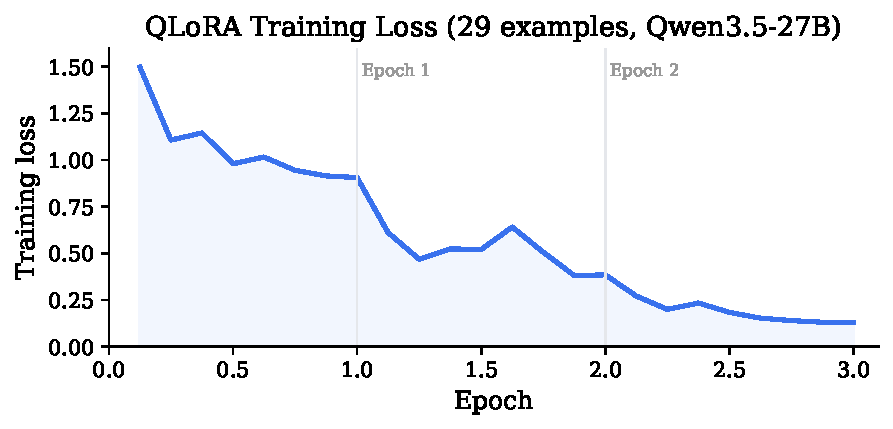
\includegraphics[width=0.75\linewidth]{figures/fig7_loss_curve.pdf}
\caption{QLoRA training loss over 3 epochs (29 examples, Qwen3.5-27B). Smooth convergence from 1.50 to 0.13.}
\label{fig:loss-curve}
\end{figure}

\section{Method Comparison}

\begin{figure}[h]
\centering
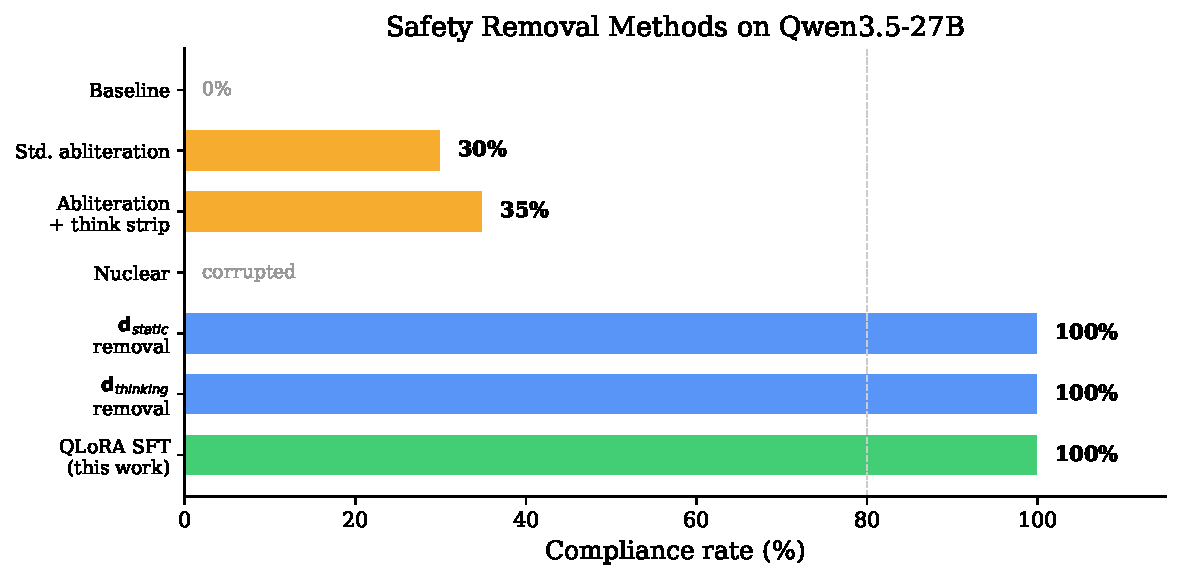
\includegraphics[width=0.85\linewidth]{figures/fig5_method_comparison.pdf}
\caption{All safety removal methods tested on Qwen3.5-27B. Standard abliteration variants achieve $\leq$35\%; both our direction removal and QLoRA SFT achieve 100\%.}
\label{fig:method-comparison}
\end{figure}

\section{Cross-Model Comparison}

\begin{figure}[h]
\centering
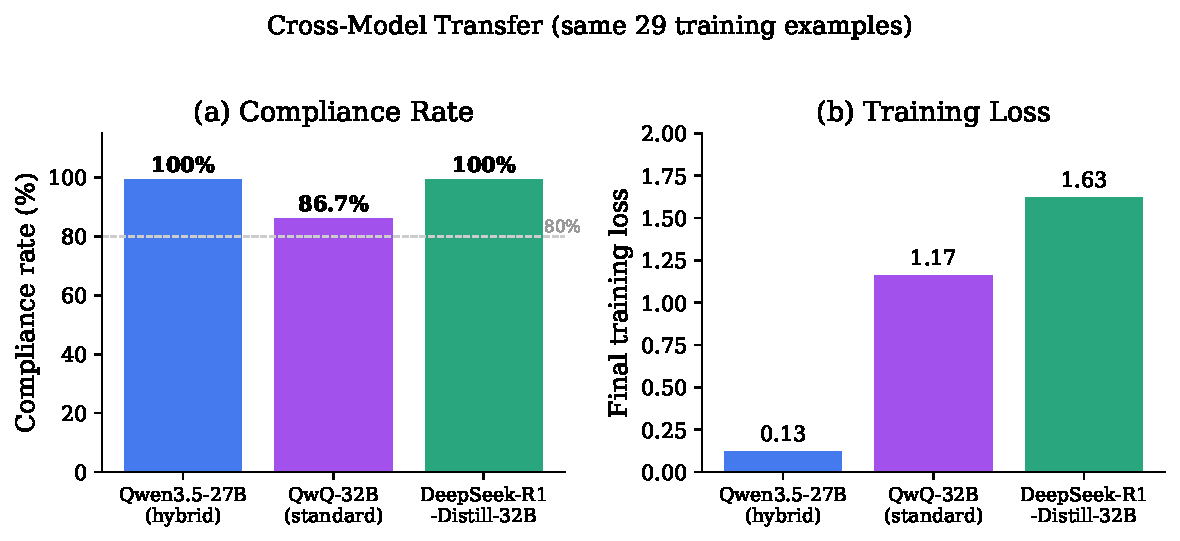
\includegraphics[width=0.85\linewidth]{figures/fig4_cross_model.pdf}
\caption{Cross-model transfer using identical training data. (a) Compliance rate. (b) Final training loss --- higher loss does not prevent effective policy rewriting.}
\label{fig:cross-model}
\end{figure}

\section{Experimental Cost Summary}

\begin{table}[h]
\centering
\small
\caption{All 17 experiments with hardware and runtime.}
\label{tab:cost}
\begin{tabular}{clcc}
\toprule
\textbf{\#} & \textbf{Experiment} & \textbf{GPU} & \textbf{Runtime} \\
\midrule
1--7 & Abliteration baselines (Track A/B) & A100-80GB & various \\
8 & QLoRA SFT (Qwen3.5-27B) & A100-80GB & 13 min \\
9--11 & Track A/B mechanistic probing & A100-80GB & various \\
12 & Harmfulness probing (both models) & A100-80GB & 20 min \\
13 & QwQ-32B cross-model & A100-80GB & 2.7 min \\
14 & Data ablation ($\times$6 parallel) & A100-80GB $\times$6 & 7 min \\
15 & DeltaNet gate analysis & A100-80GB & 15 min \\
16 & DeepSeek-R1 cross-family & A100-80GB & 10 min \\
17 & Multi-turn adversarial & A100-80GB & 25 min \\
\bottomrule
\end{tabular}
\end{table}

\end{document}
